% Created by tikzDevice version 0.9 on 2016-01-09 17:34:26
% !TEX encoding = UTF-8 Unicode
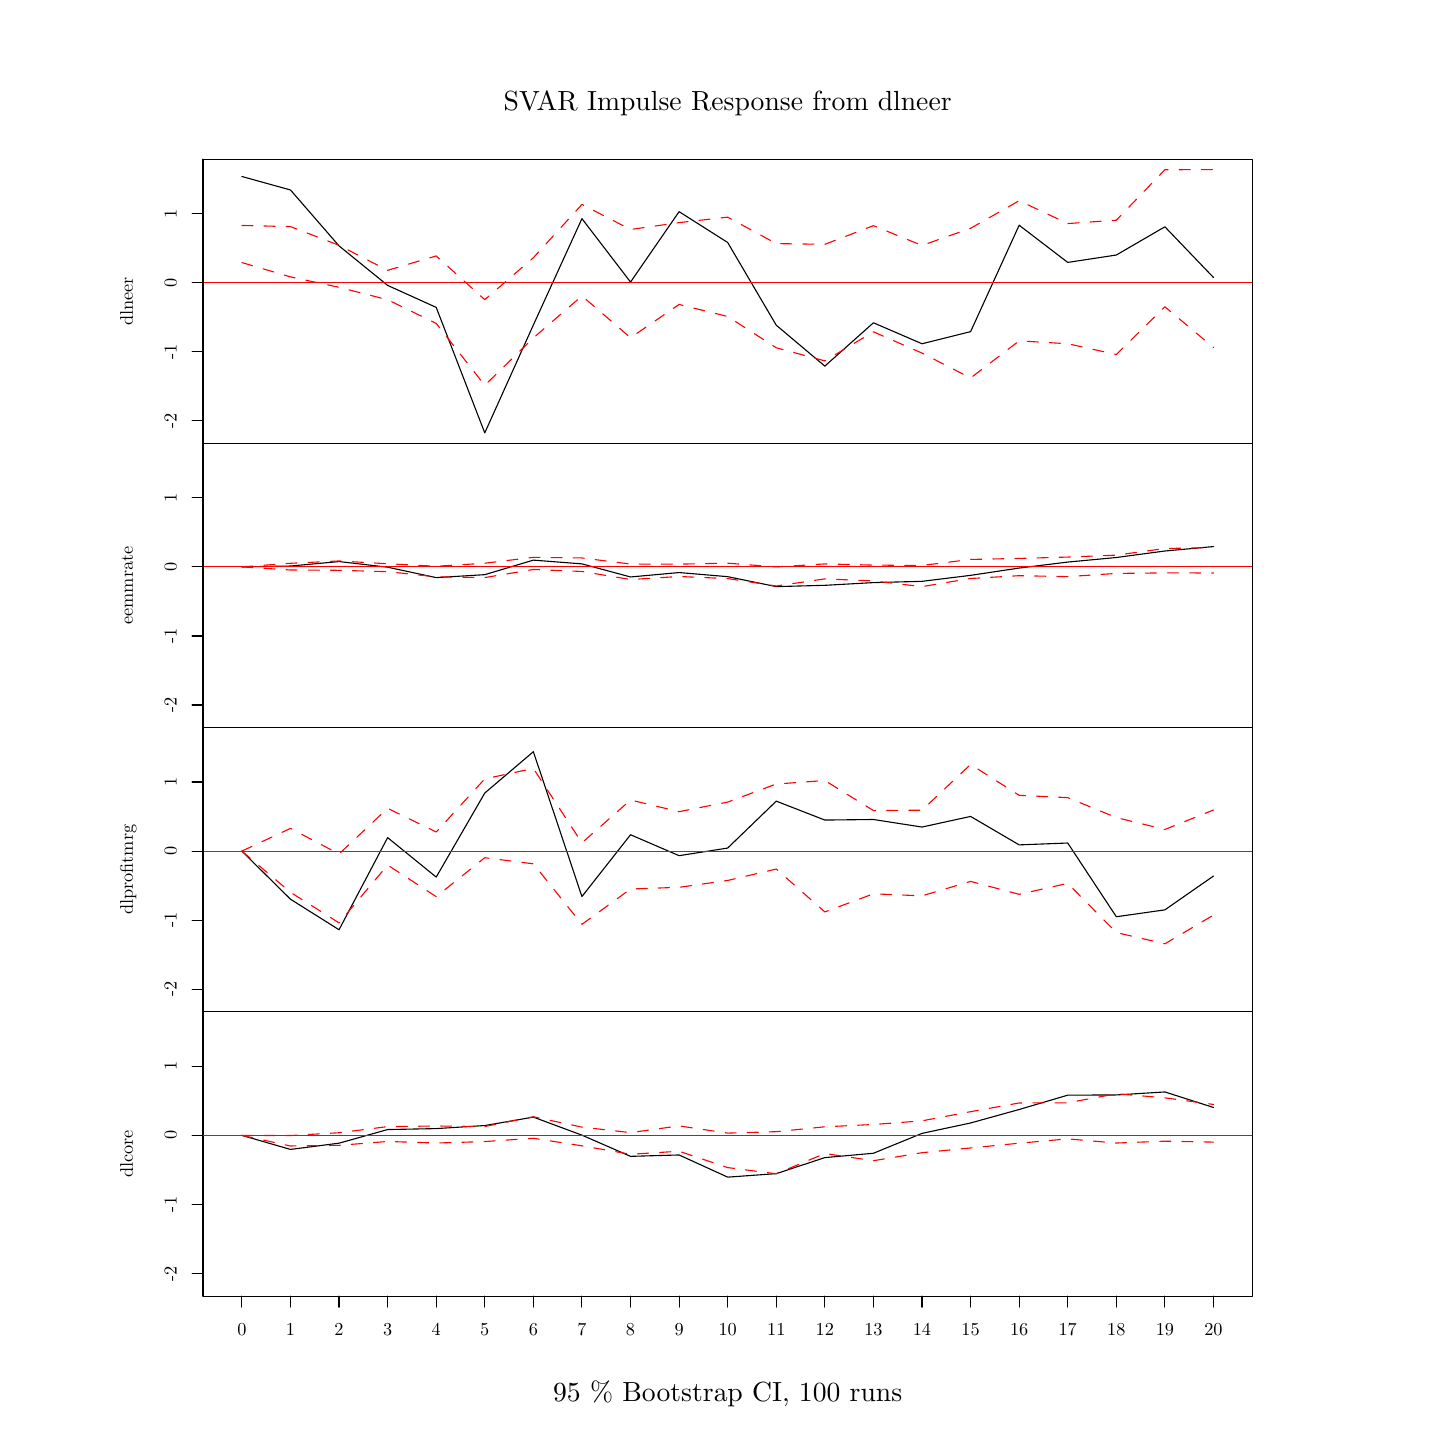
\begin{tikzpicture}[x=1pt,y=1pt]
\definecolor{fillColor}{RGB}{255,255,255}
\path[use as bounding box,fill=fillColor,fill opacity=0.00] (0,0) rectangle (505.89,505.89);
\begin{scope}
\path[clip] ( 63.36,355.66) rectangle (442.53,458.37);
\definecolor{drawColor}{RGB}{0,0,0}

\path[draw=drawColor,line width= 0.4pt,line join=round,line cap=round] ( 77.40,452.11) --
	( 94.96,447.24) --
	(112.51,427.03) --
	(130.07,412.76) --
	(147.62,404.81) --
	(165.17,359.46) --
	(182.73,398.45) --
	(200.28,436.88) --
	(217.84,413.96) --
	(235.39,439.40) --
	(252.94,428.26) --
	(270.50,398.37) --
	(288.05,383.59) --
	(305.61,399.25) --
	(323.16,391.67) --
	(340.72,396.04) --
	(358.27,434.50) --
	(375.82,421.06) --
	(393.38,423.73) --
	(410.93,433.93) --
	(428.49,415.61);
\end{scope}
\begin{scope}
\path[clip] ( 31.68,355.66) rectangle (474.21,458.37);
\definecolor{drawColor}{RGB}{0,0,0}

\node[text=drawColor,anchor=base,inner sep=0pt, outer sep=0pt, scale=  0.66] at (252.94,325.56) {xy{\$}x};

\node[text=drawColor,rotate= 90.00,anchor=base,inner sep=0pt, outer sep=0pt, scale=  0.66] at ( 38.02,407.01) {dlneer};
\end{scope}
\begin{scope}
\path[clip] (  0.00,  0.00) rectangle (505.89,505.89);
\definecolor{drawColor}{RGB}{0,0,0}

\path[draw=drawColor,line width= 0.4pt,line join=round,line cap=round] ( 63.36,363.83) -- ( 63.36,458.37);

\path[draw=drawColor,line width= 0.4pt,line join=round,line cap=round] ( 63.36,363.83) -- ( 59.40,363.83);

\path[draw=drawColor,line width= 0.4pt,line join=round,line cap=round] ( 63.36,388.80) -- ( 59.40,388.80);

\path[draw=drawColor,line width= 0.4pt,line join=round,line cap=round] ( 63.36,413.76) -- ( 59.40,413.76);

\path[draw=drawColor,line width= 0.4pt,line join=round,line cap=round] ( 63.36,438.72) -- ( 59.40,438.72);

\node[text=drawColor,rotate= 90.00,anchor=base,inner sep=0pt, outer sep=0pt, scale=  0.66] at ( 53.86,363.83) {-2};

\node[text=drawColor,rotate= 90.00,anchor=base,inner sep=0pt, outer sep=0pt, scale=  0.66] at ( 53.86,388.80) {-1};

\node[text=drawColor,rotate= 90.00,anchor=base,inner sep=0pt, outer sep=0pt, scale=  0.66] at ( 53.86,413.76) {0};

\node[text=drawColor,rotate= 90.00,anchor=base,inner sep=0pt, outer sep=0pt, scale=  0.66] at ( 53.86,438.72) {1};
\end{scope}
\begin{scope}
\path[clip] ( 63.36,355.66) rectangle (442.53,458.37);
\definecolor{drawColor}{RGB}{255,0,0}

\path[draw=drawColor,line width= 0.4pt,line join=round,line cap=round] ( 63.36,413.76) -- (442.53,413.76);

\path[draw=drawColor,line width= 0.4pt,dash pattern=on 4pt off 4pt ,line join=round,line cap=round] ( 77.40,434.41) --
	( 94.96,434.00) --
	(112.51,427.24) --
	(130.07,418.20) --
	(147.62,423.40) --
	(165.17,407.61) --
	(182.73,422.75) --
	(200.28,442.01) --
	(217.84,432.96) --
	(235.39,435.44) --
	(252.94,437.41) --
	(270.50,427.86) --
	(288.05,427.60) --
	(305.61,434.34) --
	(323.16,427.19) --
	(340.72,433.39) --
	(358.27,443.35) --
	(375.82,435.10) --
	(393.38,436.31) --
	(410.93,454.56) --
	(428.49,454.57);

\path[draw=drawColor,line width= 0.4pt,dash pattern=on 4pt off 4pt ,line join=round,line cap=round] ( 77.40,421.00) --
	( 94.96,415.83) --
	(112.51,412.07) --
	(130.07,407.57) --
	(147.62,399.03) --
	(165.17,376.64) --
	(182.73,393.78) --
	(200.28,408.95) --
	(217.84,393.85) --
	(235.39,405.87) --
	(252.94,401.52) --
	(270.50,390.21) --
	(288.05,385.48) --
	(305.61,395.98) --
	(323.16,388.30) --
	(340.72,379.30) --
	(358.27,392.71) --
	(375.82,391.68) --
	(393.38,387.78) --
	(410.93,405.03) --
	(428.49,390.32);
\end{scope}
\begin{scope}
\path[clip] (  0.00,  0.00) rectangle (505.89,505.89);
\definecolor{drawColor}{RGB}{0,0,0}

\path[draw=drawColor,line width= 0.4pt,line join=round,line cap=round] ( 63.36,355.66) --
	(442.53,355.66) --
	(442.53,458.37) --
	( 63.36,458.37) --
	( 63.36,355.66);
\end{scope}
\begin{scope}
\path[clip] ( 63.36,252.94) rectangle (442.53,355.66);
\definecolor{drawColor}{RGB}{0,0,0}

\path[draw=drawColor,line width= 0.4pt,line join=round,line cap=round] ( 77.40,311.05) --
	( 94.96,311.35) --
	(112.51,312.96) --
	(130.07,310.93) --
	(147.62,307.16) --
	(165.17,308.23) --
	(182.73,313.48) --
	(200.28,312.13) --
	(217.84,307.40) --
	(235.39,308.99) --
	(252.94,307.51) --
	(270.50,303.91) --
	(288.05,304.38) --
	(305.61,305.36) --
	(323.16,305.82) --
	(340.72,307.98) --
	(358.27,310.62) --
	(375.82,312.78) --
	(393.38,314.43) --
	(410.93,316.78) --
	(428.49,318.38);
\end{scope}
\begin{scope}
\path[clip] ( 31.68,252.94) rectangle (474.21,355.66);
\definecolor{drawColor}{RGB}{0,0,0}

\node[text=drawColor,anchor=base,inner sep=0pt, outer sep=0pt, scale=  0.66] at (252.94,222.85) {xy{\$}x};

\node[text=drawColor,rotate= 90.00,anchor=base,inner sep=0pt, outer sep=0pt, scale=  0.66] at ( 38.02,304.30) {eemmrate};
\end{scope}
\begin{scope}
\path[clip] (  0.00,  0.00) rectangle (505.89,505.89);
\definecolor{drawColor}{RGB}{0,0,0}

\path[draw=drawColor,line width= 0.4pt,line join=round,line cap=round] ( 63.36,261.12) -- ( 63.36,355.66);

\path[draw=drawColor,line width= 0.4pt,line join=round,line cap=round] ( 63.36,261.12) -- ( 59.40,261.12);

\path[draw=drawColor,line width= 0.4pt,line join=round,line cap=round] ( 63.36,286.08) -- ( 59.40,286.08);

\path[draw=drawColor,line width= 0.4pt,line join=round,line cap=round] ( 63.36,311.05) -- ( 59.40,311.05);

\path[draw=drawColor,line width= 0.4pt,line join=round,line cap=round] ( 63.36,336.01) -- ( 59.40,336.01);

\node[text=drawColor,rotate= 90.00,anchor=base,inner sep=0pt, outer sep=0pt, scale=  0.66] at ( 53.86,261.12) {-2};

\node[text=drawColor,rotate= 90.00,anchor=base,inner sep=0pt, outer sep=0pt, scale=  0.66] at ( 53.86,286.08) {-1};

\node[text=drawColor,rotate= 90.00,anchor=base,inner sep=0pt, outer sep=0pt, scale=  0.66] at ( 53.86,311.05) {0};

\node[text=drawColor,rotate= 90.00,anchor=base,inner sep=0pt, outer sep=0pt, scale=  0.66] at ( 53.86,336.01) {1};
\end{scope}
\begin{scope}
\path[clip] ( 63.36,252.94) rectangle (442.53,355.66);
\definecolor{drawColor}{RGB}{255,0,0}

\path[draw=drawColor,line width= 0.4pt,line join=round,line cap=round] ( 63.36,311.05) -- (442.53,311.05);

\path[draw=drawColor,line width= 0.4pt,dash pattern=on 4pt off 4pt ,line join=round,line cap=round] ( 77.40,311.05) --
	( 94.96,312.34) --
	(112.51,313.18) --
	(130.07,312.17) --
	(147.62,311.27) --
	(165.17,312.36) --
	(182.73,314.49) --
	(200.28,314.27) --
	(217.84,312.06) --
	(235.39,312.04) --
	(252.94,312.38) --
	(270.50,311.03) --
	(288.05,312.11) --
	(305.61,311.69) --
	(323.16,311.56) --
	(340.72,313.73) --
	(358.27,314.10) --
	(375.82,314.59) --
	(393.38,315.29) --
	(410.93,317.68) --
	(428.49,318.01);

\path[draw=drawColor,line width= 0.4pt,dash pattern=on 4pt off 4pt ,line join=round,line cap=round] ( 77.40,311.05) --
	( 94.96,309.91) --
	(112.51,309.80) --
	(130.07,309.32) --
	(147.62,307.44) --
	(165.17,307.18) --
	(182.73,310.11) --
	(200.28,309.39) --
	(217.84,306.48) --
	(235.39,307.57) --
	(252.94,306.82) --
	(270.50,304.14) --
	(288.05,306.70) --
	(305.61,305.96) --
	(323.16,303.91) --
	(340.72,306.85) --
	(358.27,307.86) --
	(375.82,307.52) --
	(393.38,308.68) --
	(410.93,308.87) --
	(428.49,308.84);
\end{scope}
\begin{scope}
\path[clip] (  0.00,  0.00) rectangle (505.89,505.89);
\definecolor{drawColor}{RGB}{0,0,0}

\path[draw=drawColor,line width= 0.4pt,line join=round,line cap=round] ( 63.36,252.94) --
	(442.53,252.94) --
	(442.53,355.66) --
	( 63.36,355.66) --
	( 63.36,252.94);
\end{scope}
\begin{scope}
\path[clip] ( 63.36,150.23) rectangle (442.53,252.94);
\definecolor{drawColor}{RGB}{0,0,0}

\path[draw=drawColor,line width= 0.4pt,line join=round,line cap=round] ( 77.40,208.34) --
	( 94.96,190.96) --
	(112.51,179.92) --
	(130.07,213.21) --
	(147.62,198.95) --
	(165.17,229.32) --
	(182.73,244.26) --
	(200.28,191.92) --
	(217.84,214.25) --
	(235.39,206.69) --
	(252.94,209.44) --
	(270.50,226.39) --
	(288.05,219.56) --
	(305.61,219.76) --
	(323.16,217.03) --
	(340.72,220.87) --
	(358.27,210.59) --
	(375.82,211.26) --
	(393.38,184.62) --
	(410.93,187.11) --
	(428.49,199.33);
\end{scope}
\begin{scope}
\path[clip] ( 31.68,150.23) rectangle (474.21,252.94);
\definecolor{drawColor}{RGB}{0,0,0}

\node[text=drawColor,anchor=base,inner sep=0pt, outer sep=0pt, scale=  0.66] at (252.94,120.14) {xy{\$}x};

\node[text=drawColor,rotate= 90.00,anchor=base,inner sep=0pt, outer sep=0pt, scale=  0.66] at ( 38.02,201.59) {dlprofitmrg};
\end{scope}
\begin{scope}
\path[clip] (  0.00,  0.00) rectangle (505.89,505.89);
\definecolor{drawColor}{RGB}{0,0,0}

\path[draw=drawColor,line width= 0.4pt,line join=round,line cap=round] ( 63.36,158.41) -- ( 63.36,252.95);

\path[draw=drawColor,line width= 0.4pt,line join=round,line cap=round] ( 63.36,158.41) -- ( 59.40,158.41);

\path[draw=drawColor,line width= 0.4pt,line join=round,line cap=round] ( 63.36,183.37) -- ( 59.40,183.37);

\path[draw=drawColor,line width= 0.4pt,line join=round,line cap=round] ( 63.36,208.34) -- ( 59.40,208.34);

\path[draw=drawColor,line width= 0.4pt,line join=round,line cap=round] ( 63.36,233.30) -- ( 59.40,233.30);

\node[text=drawColor,rotate= 90.00,anchor=base,inner sep=0pt, outer sep=0pt, scale=  0.66] at ( 53.86,158.41) {-2};

\node[text=drawColor,rotate= 90.00,anchor=base,inner sep=0pt, outer sep=0pt, scale=  0.66] at ( 53.86,183.37) {-1};

\node[text=drawColor,rotate= 90.00,anchor=base,inner sep=0pt, outer sep=0pt, scale=  0.66] at ( 53.86,208.34) {0};

\node[text=drawColor,rotate= 90.00,anchor=base,inner sep=0pt, outer sep=0pt, scale=  0.66] at ( 53.86,233.30) {1};
\end{scope}
\begin{scope}
\path[clip] ( 63.36,150.23) rectangle (442.53,252.94);
\definecolor{drawColor}{RGB}{255,0,0}

\path[draw=drawColor,line width= 0.4pt,line join=round,line cap=round] ( 63.36,208.34) -- (442.53,208.34);

\path[draw=drawColor,line width= 0.4pt,dash pattern=on 4pt off 4pt ,line join=round,line cap=round] ( 77.40,208.34) --
	( 94.96,216.55) --
	(112.51,207.31) --
	(130.07,223.80) --
	(147.62,215.24) --
	(165.17,234.44) --
	(182.73,238.20) --
	(200.28,211.33) --
	(217.84,226.81) --
	(235.39,222.59) --
	(252.94,226.05) --
	(270.50,232.58) --
	(288.05,233.84) --
	(305.61,222.99) --
	(323.16,223.12) --
	(340.72,239.65) --
	(358.27,228.50) --
	(375.82,227.66) --
	(393.38,220.46) --
	(410.93,216.15) --
	(428.49,223.19);

\path[draw=drawColor,line width= 0.4pt,dash pattern=on 4pt off 4pt ,line join=round,line cap=round] ( 77.40,208.34) --
	( 94.96,193.46) --
	(112.51,182.41) --
	(130.07,203.30) --
	(147.62,191.88) --
	(165.17,205.95) --
	(182.73,203.75) --
	(200.28,181.88) --
	(217.84,194.64) --
	(235.39,195.26) --
	(252.94,197.73) --
	(270.50,201.86) --
	(288.05,186.36) --
	(305.61,192.91) --
	(323.16,192.17) --
	(340.72,197.39) --
	(358.27,192.73) --
	(375.82,196.68) --
	(393.38,178.90) --
	(410.93,174.85) --
	(428.49,185.22);
\end{scope}
\begin{scope}
\path[clip] (  0.00,  0.00) rectangle (505.89,505.89);
\definecolor{drawColor}{RGB}{0,0,0}

\path[draw=drawColor,line width= 0.4pt,line join=round,line cap=round] ( 63.36,150.23) --
	(442.53,150.23) --
	(442.53,252.94) --
	( 63.36,252.94) --
	( 63.36,150.23);
\end{scope}
\begin{scope}
\path[clip] ( 63.36, 47.52) rectangle (442.53,150.23);
\definecolor{drawColor}{RGB}{0,0,0}

\path[draw=drawColor,line width= 0.4pt,line join=round,line cap=round] ( 77.40,105.62) --
	( 94.96,100.54) --
	(112.51,102.80) --
	(130.07,107.72) --
	(147.62,108.07) --
	(165.17,109.17) --
	(182.73,112.22) --
	(200.28,105.70) --
	(217.84, 98.04) --
	(235.39, 98.54) --
	(252.94, 90.53) --
	(270.50, 91.79) --
	(288.05, 97.58) --
	(305.61, 99.16) --
	(323.16,106.34) --
	(340.72,110.10) --
	(358.27,114.97) --
	(375.82,120.15) --
	(393.38,120.23) --
	(410.93,121.31) --
	(428.49,115.70);
\end{scope}
\begin{scope}
\path[clip] ( 31.68, 47.52) rectangle (474.21,150.23);
\definecolor{drawColor}{RGB}{0,0,0}

\node[text=drawColor,anchor=base,inner sep=0pt, outer sep=0pt, scale=  0.66] at (252.94, 17.42) {xy{\$}x};

\node[text=drawColor,rotate= 90.00,anchor=base,inner sep=0pt, outer sep=0pt, scale=  0.66] at ( 38.02, 98.88) {dlcore};
\end{scope}
\begin{scope}
\path[clip] (  0.00,  0.00) rectangle (505.89,505.89);
\definecolor{drawColor}{RGB}{0,0,0}

\path[draw=drawColor,line width= 0.4pt,line join=round,line cap=round] ( 63.36, 55.69) -- ( 63.36,150.23);

\path[draw=drawColor,line width= 0.4pt,line join=round,line cap=round] ( 63.36, 55.69) -- ( 59.40, 55.69);

\path[draw=drawColor,line width= 0.4pt,line join=round,line cap=round] ( 63.36, 80.66) -- ( 59.40, 80.66);

\path[draw=drawColor,line width= 0.4pt,line join=round,line cap=round] ( 63.36,105.62) -- ( 59.40,105.62);

\path[draw=drawColor,line width= 0.4pt,line join=round,line cap=round] ( 63.36,130.59) -- ( 59.40,130.59);

\node[text=drawColor,rotate= 90.00,anchor=base,inner sep=0pt, outer sep=0pt, scale=  0.66] at ( 53.86, 55.69) {-2};

\node[text=drawColor,rotate= 90.00,anchor=base,inner sep=0pt, outer sep=0pt, scale=  0.66] at ( 53.86, 80.66) {-1};

\node[text=drawColor,rotate= 90.00,anchor=base,inner sep=0pt, outer sep=0pt, scale=  0.66] at ( 53.86,105.62) {0};

\node[text=drawColor,rotate= 90.00,anchor=base,inner sep=0pt, outer sep=0pt, scale=  0.66] at ( 53.86,130.59) {1};

\path[draw=drawColor,line width= 0.4pt,line join=round,line cap=round] ( 77.40, 47.52) -- (428.49, 47.52);

\path[draw=drawColor,line width= 0.4pt,line join=round,line cap=round] ( 77.40, 47.52) -- ( 77.40, 43.56);

\path[draw=drawColor,line width= 0.4pt,line join=round,line cap=round] ( 94.96, 47.52) -- ( 94.96, 43.56);

\path[draw=drawColor,line width= 0.4pt,line join=round,line cap=round] (112.51, 47.52) -- (112.51, 43.56);

\path[draw=drawColor,line width= 0.4pt,line join=round,line cap=round] (130.07, 47.52) -- (130.07, 43.56);

\path[draw=drawColor,line width= 0.4pt,line join=round,line cap=round] (147.62, 47.52) -- (147.62, 43.56);

\path[draw=drawColor,line width= 0.4pt,line join=round,line cap=round] (165.17, 47.52) -- (165.17, 43.56);

\path[draw=drawColor,line width= 0.4pt,line join=round,line cap=round] (182.73, 47.52) -- (182.73, 43.56);

\path[draw=drawColor,line width= 0.4pt,line join=round,line cap=round] (200.28, 47.52) -- (200.28, 43.56);

\path[draw=drawColor,line width= 0.4pt,line join=round,line cap=round] (217.84, 47.52) -- (217.84, 43.56);

\path[draw=drawColor,line width= 0.4pt,line join=round,line cap=round] (235.39, 47.52) -- (235.39, 43.56);

\path[draw=drawColor,line width= 0.4pt,line join=round,line cap=round] (252.94, 47.52) -- (252.94, 43.56);

\path[draw=drawColor,line width= 0.4pt,line join=round,line cap=round] (270.50, 47.52) -- (270.50, 43.56);

\path[draw=drawColor,line width= 0.4pt,line join=round,line cap=round] (288.05, 47.52) -- (288.05, 43.56);

\path[draw=drawColor,line width= 0.4pt,line join=round,line cap=round] (305.61, 47.52) -- (305.61, 43.56);

\path[draw=drawColor,line width= 0.4pt,line join=round,line cap=round] (323.16, 47.52) -- (323.16, 43.56);

\path[draw=drawColor,line width= 0.4pt,line join=round,line cap=round] (340.72, 47.52) -- (340.72, 43.56);

\path[draw=drawColor,line width= 0.4pt,line join=round,line cap=round] (358.27, 47.52) -- (358.27, 43.56);

\path[draw=drawColor,line width= 0.4pt,line join=round,line cap=round] (375.82, 47.52) -- (375.82, 43.56);

\path[draw=drawColor,line width= 0.4pt,line join=round,line cap=round] (393.38, 47.52) -- (393.38, 43.56);

\path[draw=drawColor,line width= 0.4pt,line join=round,line cap=round] (410.93, 47.52) -- (410.93, 43.56);

\path[draw=drawColor,line width= 0.4pt,line join=round,line cap=round] (428.49, 47.52) -- (428.49, 43.56);

\node[text=drawColor,anchor=base,inner sep=0pt, outer sep=0pt, scale=  0.66] at ( 77.40, 33.26) {0};

\node[text=drawColor,anchor=base,inner sep=0pt, outer sep=0pt, scale=  0.66] at ( 94.96, 33.26) {1};

\node[text=drawColor,anchor=base,inner sep=0pt, outer sep=0pt, scale=  0.66] at (112.51, 33.26) {2};

\node[text=drawColor,anchor=base,inner sep=0pt, outer sep=0pt, scale=  0.66] at (130.07, 33.26) {3};

\node[text=drawColor,anchor=base,inner sep=0pt, outer sep=0pt, scale=  0.66] at (147.62, 33.26) {4};

\node[text=drawColor,anchor=base,inner sep=0pt, outer sep=0pt, scale=  0.66] at (165.17, 33.26) {5};

\node[text=drawColor,anchor=base,inner sep=0pt, outer sep=0pt, scale=  0.66] at (182.73, 33.26) {6};

\node[text=drawColor,anchor=base,inner sep=0pt, outer sep=0pt, scale=  0.66] at (200.28, 33.26) {7};

\node[text=drawColor,anchor=base,inner sep=0pt, outer sep=0pt, scale=  0.66] at (217.84, 33.26) {8};

\node[text=drawColor,anchor=base,inner sep=0pt, outer sep=0pt, scale=  0.66] at (235.39, 33.26) {9};

\node[text=drawColor,anchor=base,inner sep=0pt, outer sep=0pt, scale=  0.66] at (252.94, 33.26) {10};

\node[text=drawColor,anchor=base,inner sep=0pt, outer sep=0pt, scale=  0.66] at (270.50, 33.26) {11};

\node[text=drawColor,anchor=base,inner sep=0pt, outer sep=0pt, scale=  0.66] at (288.05, 33.26) {12};

\node[text=drawColor,anchor=base,inner sep=0pt, outer sep=0pt, scale=  0.66] at (305.61, 33.26) {13};

\node[text=drawColor,anchor=base,inner sep=0pt, outer sep=0pt, scale=  0.66] at (323.16, 33.26) {14};

\node[text=drawColor,anchor=base,inner sep=0pt, outer sep=0pt, scale=  0.66] at (340.72, 33.26) {15};

\node[text=drawColor,anchor=base,inner sep=0pt, outer sep=0pt, scale=  0.66] at (358.27, 33.26) {16};

\node[text=drawColor,anchor=base,inner sep=0pt, outer sep=0pt, scale=  0.66] at (375.82, 33.26) {17};

\node[text=drawColor,anchor=base,inner sep=0pt, outer sep=0pt, scale=  0.66] at (393.38, 33.26) {18};

\node[text=drawColor,anchor=base,inner sep=0pt, outer sep=0pt, scale=  0.66] at (410.93, 33.26) {19};

\node[text=drawColor,anchor=base,inner sep=0pt, outer sep=0pt, scale=  0.66] at (428.49, 33.26) {20};

\path[draw=drawColor,line width= 0.4pt,line join=round,line cap=round] ( 63.36, 47.52) --
	(442.53, 47.52) --
	(442.53,150.23) --
	( 63.36,150.23) --
	( 63.36, 47.52);
\end{scope}
\begin{scope}
\path[clip] ( 63.36, 47.52) rectangle (442.53,150.23);
\definecolor{drawColor}{RGB}{255,0,0}

\path[draw=drawColor,line width= 0.4pt,line join=round,line cap=round] ( 63.36,105.62) -- (442.53,105.62);

\path[draw=drawColor,line width= 0.4pt,dash pattern=on 4pt off 4pt ,line join=round,line cap=round] ( 77.40,105.62) --
	( 94.96,105.56) --
	(112.51,106.57) --
	(130.07,108.79) --
	(147.62,109.01) --
	(165.17,108.82) --
	(182.73,112.35) --
	(200.28,108.60) --
	(217.84,106.62) --
	(235.39,109.04) --
	(252.94,106.44) --
	(270.50,106.96) --
	(288.05,108.72) --
	(305.61,109.55) --
	(323.16,110.87) --
	(340.72,114.18) --
	(358.27,117.33) --
	(375.82,117.39) --
	(393.38,120.65) --
	(410.93,119.19) --
	(428.49,116.79);

\path[draw=drawColor,line width= 0.4pt,dash pattern=on 4pt off 4pt ,line join=round,line cap=round] ( 77.40,105.62) --
	( 94.96,101.79) --
	(112.51,102.02) --
	(130.07,103.42) --
	(147.62,102.85) --
	(165.17,103.38) --
	(182.73,104.58) --
	(200.28,101.85) --
	(217.84, 98.80) --
	(235.39, 99.88) --
	(252.94, 93.98) --
	(270.50, 91.74) --
	(288.05, 99.06) --
	(305.61, 96.47) --
	(323.16, 99.36) --
	(340.72,101.07) --
	(358.27,102.79) --
	(375.82,104.35) --
	(393.38,102.85) --
	(410.93,103.52) --
	(428.49,103.19);
\end{scope}
\begin{scope}
\path[clip] (  0.00,  0.00) rectangle (505.89,505.89);
\definecolor{drawColor}{RGB}{0,0,0}

\node[text=drawColor,anchor=base,inner sep=0pt, outer sep=0pt, scale=  1.00] at (252.94,475.79) {SVAR Impulse Response from dlneer};

\node[text=drawColor,anchor=base,inner sep=0pt, outer sep=0pt, scale=  1.00] at (252.94,  9.50) {95 {\%} Bootstrap CI,  100 runs};
\end{scope}
\end{tikzpicture}
